\documentclass[11pt,twocolumn]{article}

\usepackage[utf8]{inputenc}
\usepackage[english]{babel}
\usepackage{graphicx}
\usepackage{subfigure}
\usepackage{setspace}
\setlength{\columnseprule}{1pt}

\onehalfspacing
\begin{document}

\title{SVM Hank: A Study on Using Support Vector Machines and Textural Features to Classify Images}
\author{Heikki Salo}

\maketitle

\section{Introduction}\label{introduction}

The purpose of this study is to test image classification by preparing
adequate implementations of two common techniques used in the field of
machine vision: support vector machines and textural features.
Motivation for this test is the development of algorithms for UASI project:
multidisciplinary research project employing several technologies from
the fields of machine vision and classification.
In order to gain better understanding of new tools I'm conducting this
testing with artificial dataset (described in detail in \ref{sec_materials})
that produces easily interpretable results.

The classifying process will consist of six steps:
(1) defining the datasets for training and testing,
(2) extracting textural features from images,
(3) scaling the data,
(4) generating model using training data,
(5) predicting classes of test data and finally
(6) analyzing the results.
More details of the process are given in \ref{sec_methods}.

The study is carried out with tool called \textit{SVM Hank} \cite{hank}.
Source code of SVM Hank and other materials are available at
\texttt{http://github.com/deggis/svmhank/}.


\section{Materials}\label{sec_materials}

Images in this test are prepared using texture samples from
Trygve Randen's Brodatz Texture collection \cite{brodatz}.
Manually prepared datasets are images with dimensions of
100 px x 100 px and contain two different texture types.
Training and test datas are locations of 10 px x 10 px areas
for both texture types.
So essentially each dataset is collection of 10 px x 10 px images,
given as bigger image and a set of coordinates.

\begin{figure}[htb]
\centering
\setlength\fboxsep{0pt}
\setlength\fboxrule{1pt}
\fbox{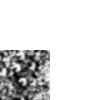
\includegraphics[width=0.2\textwidth]{level01.png}}
\caption{Case 1: Cloud texture on solid white background}
\label{fig:level1}
\end{figure}

First case (Figure \ref{fig:level1}) is simply constant
background with added texture in the corner.
Hypothesis is that this case doesn't require usage of textures
since differences in block averages could be sufficient to
separate images.

\begin{figure}[htb]
\centering
\setlength\fboxsep{0pt}
\setlength\fboxrule{1pt}
\fbox{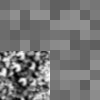
\includegraphics[width=0.2\textwidth]{level02.png}}
\caption{Case 2: Cloud texture on solid colored tiles with variating gray level and same average as texture's}
\label{fig:level2}
\end{figure}

Second case is derived from the first.
White background is darkened to gray tiles that in average match texture's average
brightness (0.4707) and has considerably higher standard distribution (0.5362) than texture's
tiles (0.1123).
Succesful classification will now require the use of textural features.

\begin{figure}[htb]
\centering
\setlength\fboxsep{0pt}
\setlength\fboxrule{1pt}
\fbox{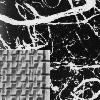
\includegraphics[width=0.2\textwidth]{level03.png}}
\caption{Case 3: Cloud texture on solid colored tiles with variating gray level and same average as texture's}
\label{fig:level3}
\end{figure}

\begin{figure}[htb]
\centering
\setlength\fboxsep{0pt}
\setlength\fboxrule{1pt}
\fbox{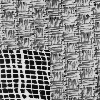
\includegraphics[width=0.2\textwidth]{level04.png}}
\caption{Case 4: High contrast web on some kind of coarse surface}
\label{fig:level4}
\end{figure}

\begin{figure}[htb]
\centering
\setlength\fboxsep{0pt}
\setlength\fboxrule{1pt}
\fbox{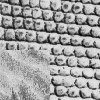
\includegraphics[width=0.2\textwidth]{level05.png}}
\caption{Case 5: Sand on snake skin}
\label{fig:level5}
\end{figure}

Cases from three through five (Figures
\ref{fig:level3},
\ref{fig:level4} and
\ref{fig:level5})
are images where both textures are more vivid than solid colors.
In case 5 there's gray regions with much similarities in both
textures which will cause trouble separating the regions
succesfully.



\section{Methods}\label{sec_methods}

For each case,
the training data is a set of 20 known locations
in the image,
containing 10 samples of both texture types.
The given coordinates are upper left corners to non-overlapping
10 px x 10 px subimages.

Datasets are processed using \emph{SVM Hank} \cite{hank},
available at \texttt{http://yousource.it.jyu.fi/svmhank/}.
SVM Hank is developed solely for solving classification
challenges of this paper.

I developed SVM Hank with Haskell programming language using
Intel's \emph{OpenCV} \cite{opencv} machine vision library.
Chih-Chung Chang's and Chih-Jen Lin's \emph{libsvm}
\cite{libsvm} is used as Support Vector Machine implementation.
Both implementations are used through Haskell packages
\emph{CV} \cite{aleator_cv} and \emph{Simple-SVM} \cite{aleator_svm}
developed by Ville Tirronen.

As summarized in \ref{introduction},
overall process consists of six steps.
After \textbf{defining the datasets (1) for training and testing},
SVM Hank carries out steps from two through five
and produces images of classification results.

Using the same training data two different methods to classify
images are tried, producing two different results.
First method is to split the full 100 px x 100 px image to
100 subimages with 10 px x 10 px of size and then predicting
classes of each.
Second method is to crop 11 px x 11 px subimages for
\emph{each pixel}
which takes the surroundings into account better.
The second method requires classifying of each 8100 subimages
and leaves 5 px thick borders out of the 90 px x 90 px
result.

The two different methods could well produce different kind of
results
since the subimage size is different.
Also in case 5 there are gray areas somewhat 10 pixels in diameter
in both class regions.

SVM Hank \textbf{extracts following features (2)} from image blocks:
\begin{itemize}
    \item average brightness
    \item angular second moments (*) and
    \item contrasts (*).
\end{itemize}

Last two features (marked with (*)) are extracted by first generating
a spatial gray tone co-occurrence matrix as described in \cite{haralick73}
with distance (lag) of 1 pixel and using angles
$0 ^{\circ}$, $45 ^{\circ}$, $90 ^{\circ}$ and $135 ^{\circ}$.
The four matrices that describe which gray tones occur as neighbours
are then used to calculate angular second moment and contrast features.
As SVM classification benefits from using many features and the orientation
of the textures is static,
the different angles are included in processing.

SVM Hank \textbf{scales the extracted feature values (3)}
to range [0,1] as recommended
in \cite{libsvm_guide}.
The training is first performed to training data to each feature
and same scaling weights are later used to test data.

\textbf{SVM model of the case is generated (4)} using the training data
and cross-validated.
With the model SVM Hank carries out the two methods to split the
image and \textbf{predicts the classes of the resulting subimages (5)}.

\textbf{SVM Hank produces result images of the two methods (6)},
which --- ideally --- both should be white images with black box in
lower left corner.

Some misclassfications are expected simply because there are regions
both texture class regions (like in case 5).
The selected two methods consist of straightforward splitting the image
to subimages.

\textbf{The compromises in this test} setup lie in the selection of texture
extraction methods and usage of SVM.
No other machine vision techniques are applied to improve results.
More possibilities are considered in section \ref{discussion}.

\section{Results}

Classification results are shown in table \ref{resulttable}.
The performance of the selected few textural features and unoptimized
SVM was surprisingly good.

For cases 1 through 5 the two methods were applied using randomly
selected SVM classification parameters $C=1$ and $\gamma=1$.
Cases 1, 3 and 4 performed well with these settings,
but for Case 5 the SVM parameters were optimized using grid
search as guided in \cite{libsvm_guide}.
With Case 5's training data grid search algorithm suggested
optimal parameters to be $C=2048.0$ and $\gamma=0.0078125$,
which improved classification accuracy from 67 \% to 88 \% in
using method 1 (Case 5b).

While classification accuracy in Case 5 could be improved
with utilizing more textural features, the Case 2
suffers from poorly selected training data.
The training data consists of the first ten non-overlapping
10 px x 10 px blocks of each region which doesn't
give clues about the real structure of the tile background.
It's clearly seen that method 2 finds familiar spots from
the background in the middle of the squares but 
gets lost near the edges.

\begin{figure}[htb]
\centering
\setlength\fboxsep{0pt}
\setlength\fboxrule{1pt}
\fbox{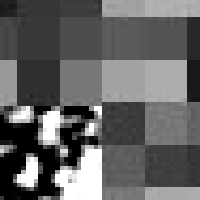
\includegraphics[width=0.2\textwidth]{level02_noise.png}}
\caption{Noise in JPEG compressed Case 2 image (enhanced contrast).}
\label{fig:level2_noise}
\end{figure}

Other unexpected issue that was related to Cases 1 and 2
and was caused by low quality JPEG compression
that resulted noise in picture.
With method 1 this noise caused some misclassification in
Case 1 and completely ruined accuracy Case 2
(although optimizing SVM parameters could've helped a bit).
This was solved by preparing original images as non-compressed
bitmaps.



\section{Discussion}\label{discussion}

In this study the used techniques --
spatial gray-tone co-occurrence textural features and support
vector machines -- were taken off-the-shelf and almost no effort
was put into optimizing parameters.
The goal was to prepare adequate implementations of selected
methods and use them in a fixed context to get easily
interpretable results.





\begin{table*}[ht]

\caption{Classification results}\label{resulttable}
\centering
\begin{tabular}{c|c|cc|cc}
\textbf{Original image} & \textbf{Original image} & \textbf{Method 1} & \textbf{Acc. (\%)} & \textbf{Method 2} & \textbf{Acc. (\%)} \\
\hline
Case 1 & 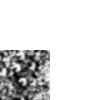
\includegraphics[scale=1]{level01.png} & 
\includegraphics[scale=1]{level01_method1.png} & 100.0 \% & 
\includegraphics[scale=1]{level01_method2.png} & 98.01 \% \\
\hline
Case 2 & 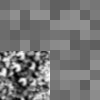
\includegraphics[scale=1]{level02.png} & 
\includegraphics[scale=1]{level02_method1.png} & 100.0 \% & 
\includegraphics[scale=1]{level02_method2.png} & 39.11 \% (!)\\
\hline
Case 3 & 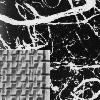
\includegraphics[scale=1]{level03.png} & 
\includegraphics[scale=1]{level03_method1.png} & 98.0 \% & 
\includegraphics[scale=1]{level03_method2.png} & 96.99 \% \\
\hline
Case 4 & 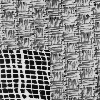
\includegraphics[scale=1]{level04.png} & 
\includegraphics[scale=1]{level04_method1.png} & 99.0 \% & 
\includegraphics[scale=1]{level04_method2.png} & 98.97 \% \\
\hline
Case 5 & 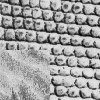
\includegraphics[scale=1]{level05.png} & 
\includegraphics[scale=1]{level05_method1.png} & 67.0 \% & 
\includegraphics[scale=1]{level05_method2.png} & 73.70 \% \\
\hline
Case 5b & 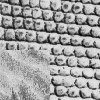
\includegraphics[scale=1]{level05_b.png} & 
\includegraphics[scale=1]{level05_b_method1.png} & 88.0 \% (!) & 
\includegraphics[scale=1]{level05_b_method2.png} & 87.36 \% \\

\end{tabular}
\label{tab:gt}

\end{table*}%


\begin{thebibliography}{55}

\bibitem{hank}
    H. Salo,
    \emph{SVM Hank},
    available at \texttt{http://github.com/deggis/svmhank/},
    2011.

\bibitem{brodatz}
    T. Randen,
    \emph{Brodatz Textures},
    available at \texttt{http://www.ux.uis.no/$\sim$tranden/\\brodatz.html}.

\bibitem{haralick73}
    R. Haralick, K. Shanmugam, I. Dinstein,
    \emph{Textural Features for Image Classification},
    IEEE Transactions on Systems, Man and Cybernetics,
    1973.

\bibitem{opencv}
    Intel Corporation,
    \emph{OpenCV: Open Source Computer Vision},
    available at \texttt{http://opencv.willowgarage.com/wiki/}.

\bibitem{libsvm}
    C. Chang, C. Lin,
    \emph{libsvm: A Library for Support Vector Machines},
    available at \texttt{http://www.csie.ntu.edu.tw/\\ $\sim$cjlin/libsvm/}.

\bibitem{aleator_cv}
    V. Tirronen,
    \emph{Haskell wrappers and utilities for OpenCV machine vision library},
    available at \texttt{https://github.com/aleator/CV/}.

\bibitem{aleator_svm}
    V. Tirronen,
    \emph{Simple SVM: Haskell bindings for libsvm},
    available at \texttt{https://github.com/aleator/CV/}.

\bibitem{libsvm_guide}
    C. Hsu, C. Chang, C. Lin,
    \emph{A Practical Guide to Support Vector Classification},
    National Taiwan University,
    Taiwan,
    2003.

\end{thebibliography}


\end{document}
